\section{DFD Design}

\subsection{External Entities, Processes, and Data Stores}

\textbf{External Entities}
\begin{itemize}
    \item Consumer
    \item Smart Meter (ESP32)
    \item Grid Administrator
\end{itemize}

\textbf{Main Processes}
\begin{itemize}
    \item Receive Meter Data
    \item Process Energy Consumption
    \item Execute Smart Contract Billing
    \item Detect Anomalies and Predict Usage
    \item Update Dashboard and Notifications
\end{itemize}

\textbf{Data Stores}
\begin{itemize}
    \item D1 Consumer Database
    \item D2 Energy Usage Database
    \item D3 Blockchain Ledger
    \item D4 Machine Learning Models
\end{itemize}

\subsection{Level 0 DFD}

The Level 0 DFD presents the overall context of the Decentralized Smart Power Grid System. Smart meters provide energy consumption data to the system. Consumers recharge prepaid balances and view usage information, while administrators monitor the system and receive alerts.

\begin{center}
    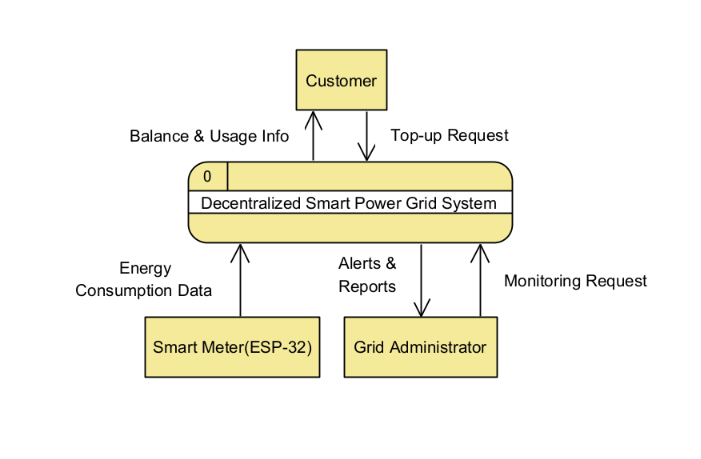
\includegraphics[width=0.7\textwidth]{graphics/level0.png}

    \small\textbf{Figure 1:} Level 0 DFD of the Decentralized Smart Power Grid System
\end{center}

\newpage

\subsection{Level 1 DFD}

The Level 1 DFD expands the system into its five major processes: receiving telemetry data, processing energy consumption, executing blockchain-based billing, detecting anomalies and updating the dashboard.

\begin{center}
    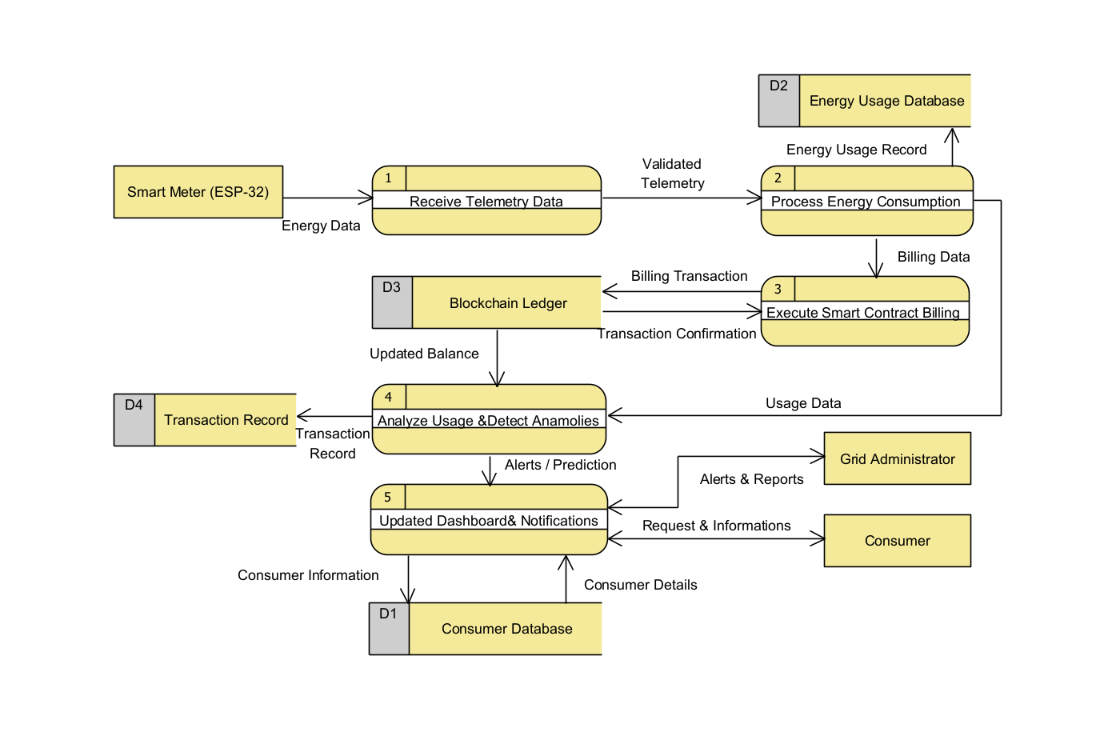
\includegraphics[width=\textwidth,height=0.75\textheight,keepaspectratio]{graphics/level1.png}

    \small\textbf{Figure 2:} Level 1 DFD of the Decentralized Smart Power Grid System
\end{center}

\newpage

\subsection{Level 2 DFD for Execute Smart Contract Billing}

The Level 2 DFD expands Process 3, Execute Smart Contract Billing. It verifies the consumer wallet, calculates energy charges, executes the blockchain smart contract, updates the remaining balance, and generates billing status.

\begin{center}
    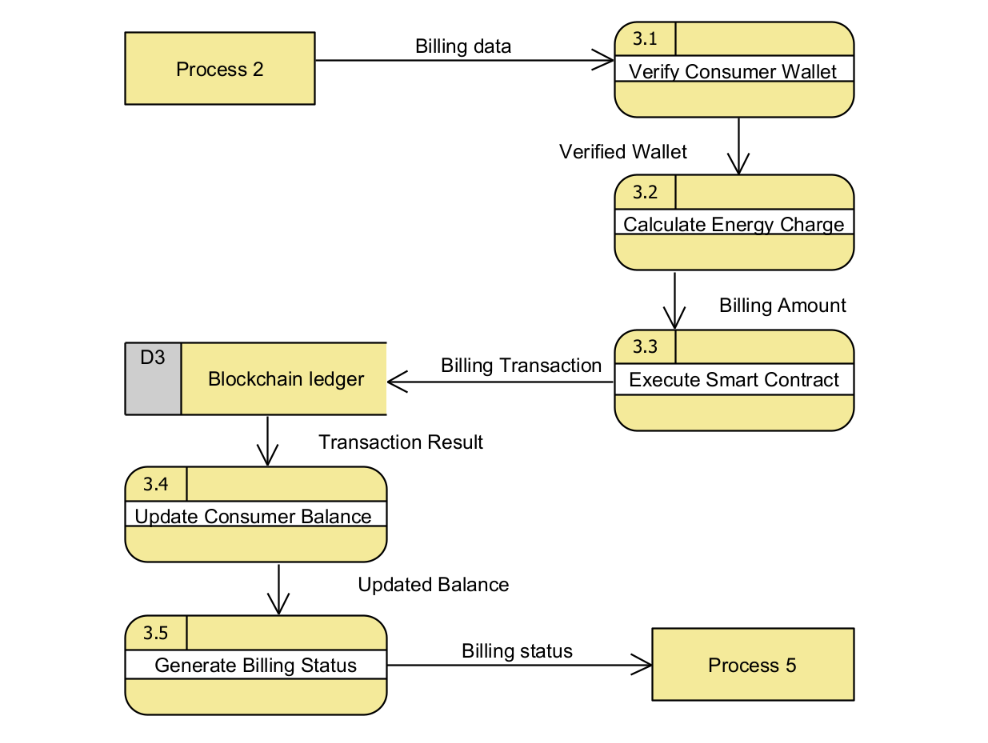
\includegraphics[width=\textwidth,height=0.75\textheight,keepaspectratio]{graphics/level2.png}

    \small\textbf{Figure 3:} Level 2 DFD for Process 3: Execute Smart Contract Billing
\end{center}

\subsection{Balancing}

The Level 2 DFD maintains the same input and output as Process 3 in the Level 1 DFD. It receives billing data from Process 2 and returns updated balance and billing status to the following processes, ensuring proper balancing between the parent and child DFDs.